\section{Experimental details}
\label{app:details}

\paragraph{World.} All bandit experiments use a bounded-Gaussian arm model: a pull of arm $i$ returns $r = \mathrm{clip}(\mathcal{N}(\mu_i,\sigma^2),0,1)$ with noise $\sigma = 0.25$. There are $N=10$ arms with means $\mu = 0.25$ on the sub-optimal arms and $\mu = 0.75$ on the single good arm. The stationary world fixes the good arm for $T = 10{,}000$ steps; the switching world runs five segments of $10{,}000$ steps and rotates the good arm at each of the four boundaries (drawn from a fixed seed). All curves report the mean over $100$ seeds with $95\%$ bootstrap intervals, and per-step regret is shown after a moving-average smoothing.

\paragraph{Agents and examiners (Figures~\ref{fig:practice_main}).} In the stationary world the well-adapted agent is UCB1 and the poorly-adapted agent is $\varepsilon$-greedy with $\varepsilon = 0.1$; the matched examiner is a full-memory Hoeffding bracket and the mismatched examiner is a sliding-window variant that assumes the world keeps changing. In the switching world the roles invert: the well-adapted agent is a reset-UCB that resets at the known boundaries and the poorly-adapted agent is UCB1; the matched examiner is reset-aware and the mismatched examiner is the full-memory bracket that assumes the world is static.

\paragraph{Capacity (Figures~\ref{fig:capacity} and \ref{fig:capacity_stationary}).} Capacity is varied by aggregating the arms into $G \in \{1,2,5,10\}$ equal groups, so the coarse party distinguishes only $G$ groups while the other stays per-arm. The agent is a sliding-window UCB and the examiner is reset-aware. In the forward setting the examiner is coarsened and the boundaries are placed so that a low-resolution examiner cannot see them; in the reverse setting the agent is coarsened and the examiner is per-arm.

\paragraph{Learner comparison (Figure~\ref{fig:learner_comparison}).} Five learners (SW-UCB, D-UCB, EXP3.S, UCB1 and Thompson sampling) are run in a switching world whose arm set grows from $10$ to $30$ across segments, each assessed by the single reset-aware examiner. The reported rank correlation is Spearman $\rho_S = 0.85$ over the $5\times100$ (learner, seed) pairs.

\section{Capacity in the stationary world}
\label{app:capacity_stationary}

We repeat the capacity probe of Section~\ref{sec:capacity} in the stationary world, where the effect is milder because there are no changes to expose a coarse examiner. Figure~\ref{fig:capacity_stationary} shows both directions. In the forward case, once the agent has identified the optimal arm the examiner's aggregation barely matters: all resolutions $G$ converge to nearly the same small $\rho^\chi_t$, since the only distinction that drives regret (optimal versus sub-optimal arm) is preserved under every grouping, with the early-transient separation visible in the inset. In the reverse case, a capacity-restricted agent again plateaus at the structural gap induced by its grouping, and the fully resolved examiner's $\rho^\chi_t$ tracks that gap from above. The stationary world therefore exercises the same mechanism as Figure~\ref{fig:capacity} but without the non-stationary stress that makes an under-resolved examiner visibly invalid.

\begin{figure}[t]
\centering
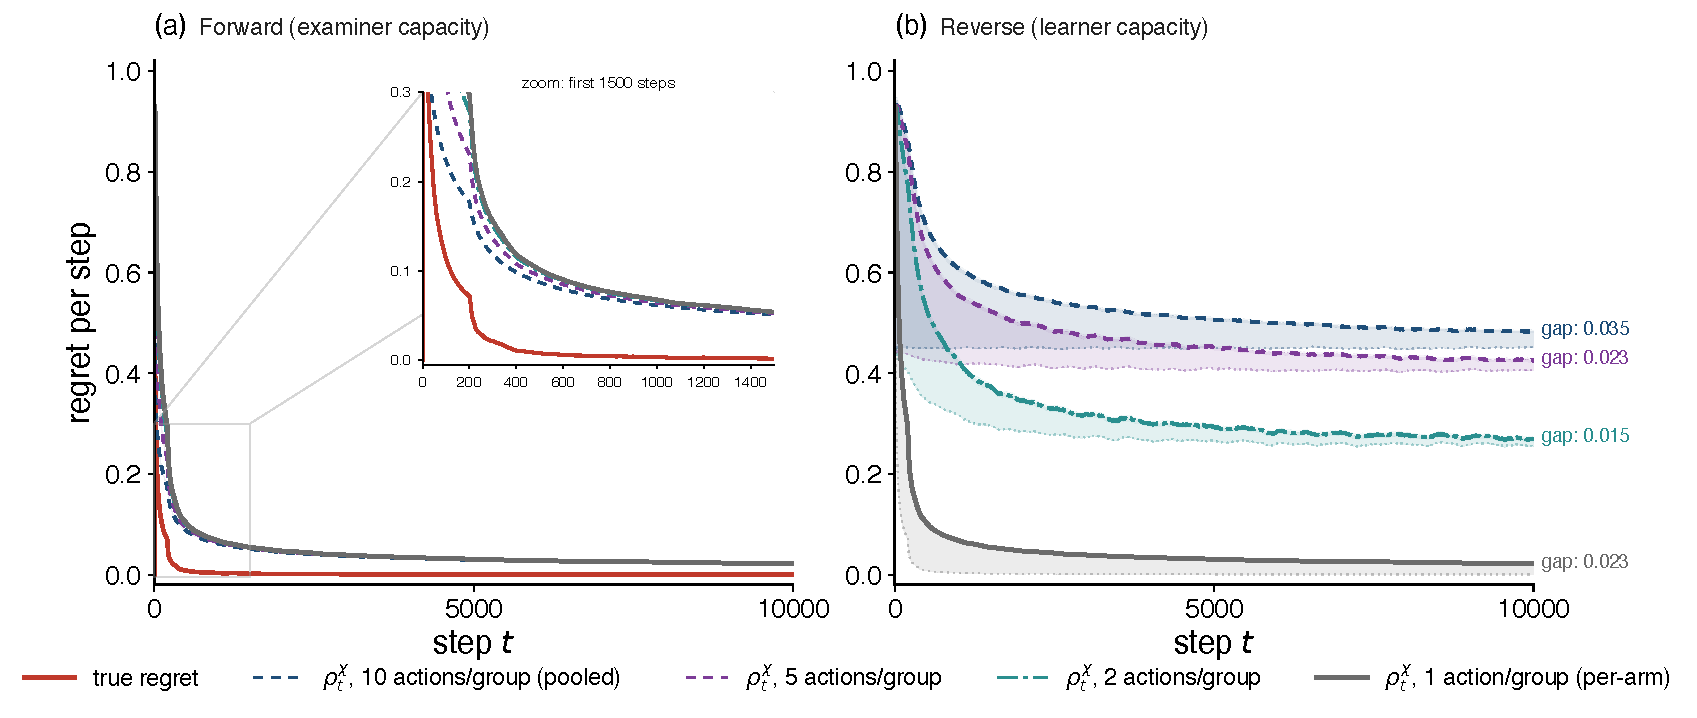
\includegraphics[width=\textwidth]{image/fig3_capacity.pdf}
\caption{Relative capacity in the stationary bandit. \textbf{(a)} Forward: a fine-grained agent assessed by an examiner that aggregates arms into $G$ groups; all $G$ converge to the same small $\rho^\chi_t$ once the optimal arm is found (inset: early transient). \textbf{(b)} Reverse: an agent restricted to $G$ groups assessed by a fully resolved examiner; $\rho^\chi_t$ plateaus just above each structural gap (labelled). Red: true regret; coloured: $\rho^\chi_t$ per $G$.}
\label{fig:capacity_stationary}
\end{figure}
